\documentclass[aspectratio=169,dvipsnames]{beamer}
\beamertemplatenavigationsymbolsempty
% \documentclass{beamer}

% UNCOMMENT FOR HANDOUTS
% \usepackage{pgfpages}
% \pgfpagesuselayout{2 on 1}[landscape,letterpaper,border shrink=5mm]
% \setbeameroption{show notes}

\mode<presentation>
\usetheme{Boadilla}
\usecolortheme{spruce}
\usepackage{../../LizStyle,ulem}
\usepackage{color}
\usepackage[color,matrix,arrow]{xy}
% \input xy
% \xyoption{all}
\usepackage{tikz}
\usepackage{tikz-cd}
\tikzset{commutative diagrams/diagrams={ampersand replacement=\&}}

\AtBeginSection{\frame{\sectionpage}}


% ==========Command for putting comments and removing them=======
% Visible:
\newcommand{\InstructorNotes}[1]{\textit{\color{orange}#1}}
\newcommand{\InstructorList}[1]{
\begin{itemize}
	\color{orange}
	#1
\end{itemize}
}
% Removed:
\renewcommand{\InstructorNotes}[1]{}
\renewcommand{\InstructorList}[1]{}


\newcommand{\bvfill}{\vskip0pt plus 1filll}

\usepackage{multimedia}
\usepackage{graphbox}

% \usepackage{algpseudocode}


\newcommand{\Reeb}{\textbf{Reeb}}
\newcommand{\Rtopc}{\textbf{Rtopc}}
% \newcommand{\RR}{\mathcal{R}}

\newcommand{\Set}{\textbf{Set}}
\newcommand{\Vect}{\textbf{Vect}}
\newcommand{\Top}{\textbf{Top}}
\newcommand{\Int}{\textbf{Int}}


\graphicspath{ {Figures/} {../Figures/}{../../Figures/} }



\begin{document}
%\pdfoptionpdfminorversion 5
%\logo{\includegraphics[height=1.5cm]{dukeshield.pdf}}
\title[Lec 2]{Ch 2.2: Assessing Model Accuracy}
\subtitle{Lecture 3 - CMSE 381}
\date{Fri, Jan 16, 2026}



\institute[MSU-CMSE]{Michigan State University\\
			::\\
          Dept of Computational Mathematics, Science \& Engineering}
%\author[Dr.~Bao]{Prof.~Lianzhang Bao}

\begin{frame}
 \titlepage


\end{frame}
%--------------------------
\begin{frame}[c]{Announcements}

\begin{columns}
\column{.35\textwidth}
\centering

	Last time:
	\begin{itemize}
		\item Ch 2.1, Vocab day!
	\end{itemize}
\column{.60\textwidth}
\centering

	Announcements: 
	\begin{itemize}
		%\item Get on slack!
		%\begin{itemize}
			%\item +1 point on the first homework if you post a gif in the thread
		%\end{itemize}
		\item First homework due Sunday, 1/25. Covers:
		\begin{itemize}
			\item Mon 1/12 lecture
			\item Weds 1/14 Lecture
			\item Today 1/16 Lecture
		\end{itemize}
		%\item Office hours!
		%\begin{itemize}
			%\item Dr.~Bao: Tue 9 am-11 am (EB 2507 L)\\
			%\item Dr.~ Khasawneh: MWF 13:40 pm-2:00 pm (EB 2400), Tue 1:30 pm-2:30 pm (Zoom)
			% (At least this week, subject to change)
			%\item Siyu : Wed 2:00 pm-3:00 pm (EB 2504)
			%\item Haishen: WF 2:00 pm-3:00 pm (EB2504)
		%\end{itemize}	
		\end{itemize}
\end{columns}

\end{frame}
%--- Next Frame ---%
\begin{frame}[c]{Covered in this lecture }

\begin{columns}
\column{.4\textwidth}
\centering
\begin{itemize}
	\item Mean Squared Error (regression)
	\item Train vs Test
	\item Bias Variance Trade off
	% \item Error rate (classification)
	% \item Bayes Classifier
	% \item $K$-NN classification
\end{itemize}
\column{.4\textwidth}
\centering

\end{columns}

\end{frame}
%--- Next Frame ---%
%--- Next Frame ---%

\begin{frame}[c]{Quick review of notation}

\begin{columns}
\column{.6\textwidth}
\centering

\InstructorList{
\item $X = (X_1,\cdots, X_p)$ number of variables
\item Ground truth $Y = f(X) + \e$
\item Approximation $\hat Y = \hat f(X)$
\item Number of data points $n$
\item $X_{ij}$ is $jth$ predictor for observation $i$
}

\column{.4\textwidth}
\centering

\end{columns}

\end{frame}
%--- Next Frame ---%
\section{Mean Squared Error}

\begin{frame}[c]{Which is better?}


\begin{columns}
\column{.6\textwidth}
\centering
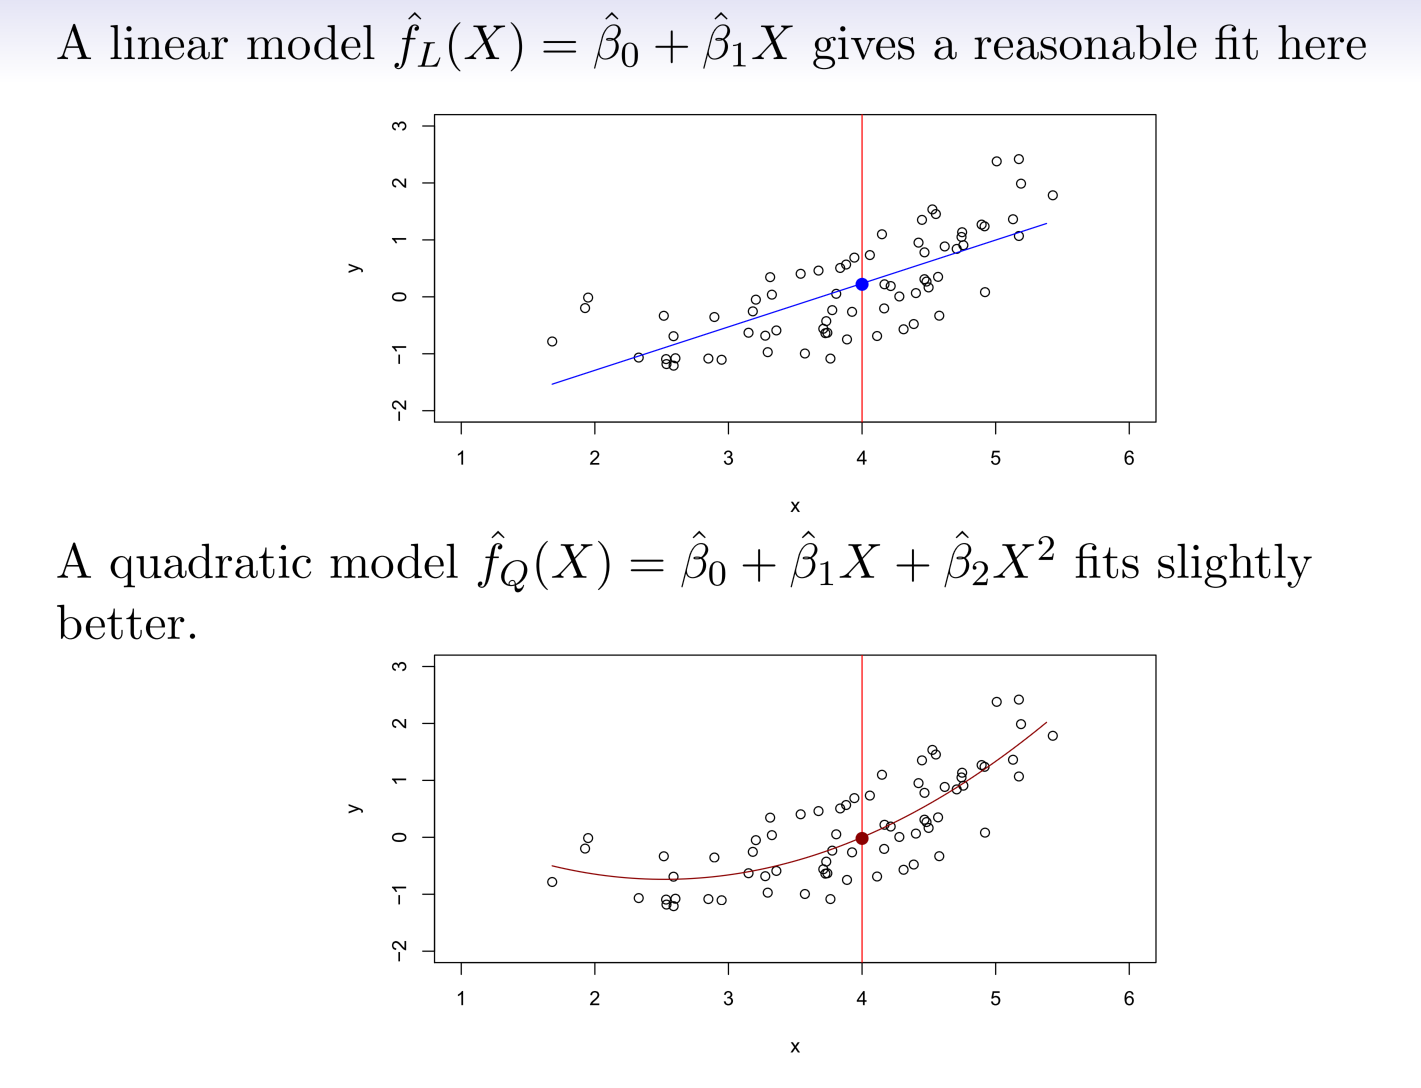
\includegraphics[alt={Two vertical scatter plots with a linear fit overlay on top and a quadratic fit overlay on bottom},width = \textwidth]{LinearVsQuadratic}

% \column{.4\textwidth}
\centering

\end{columns}

\end{frame}
%--- Next Frame ---%

\begin{frame}[c]{No free lunch}
\InstructorList{
\item No best model for all data sets
\item So, need to measure quality of a model on a given data set
}
\begin{columns}
\column{.4\textwidth}
\centering

\column{.4\textwidth}
\centering

\end{columns}

\end{frame}
%--- Next Frame ---%


\begin{frame}[t]{Mean Squared Error}
	\framesubtitle{Error in the regression setting}
\begin{equation*}
	MSE = \frac{1}{n} \sum_{i=1}^n(y_i - \hat f(x_i))^2
\end{equation*}

\centering
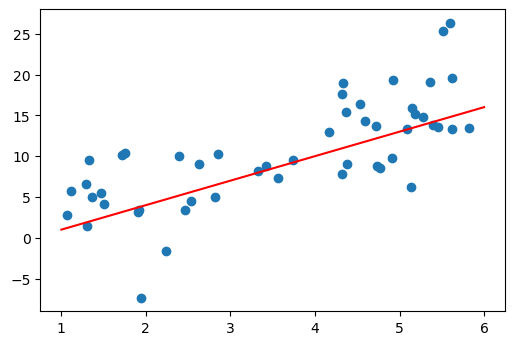
\includegraphics[alt={Planar scatter plot with a line fit to the data},width = .4\textwidth]{../Figures/ExampleLinear50pts}

\end{frame}
%--- Next Frame ---%

{
  \setbeamercolor{background canvas}{bg=Apricot!25}
\begin{frame}[t]{Group Work}

Given the following data, you decide to use the model 
\begin{equation*}
	\hat{f}(X_1,X_2) = 1-3X_1 + 2X_2.
\end{equation*}
What is the MSE?
\begin{columns}
\column{.15\textwidth}
\centering
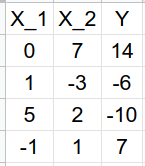
\includegraphics[alt={A data table with columns X1, X2, and Y},align = c, width = \textwidth]{FakeData-Sec2-2-MSE}

\column{.45\textwidth}
\centering
\InstructorNotes{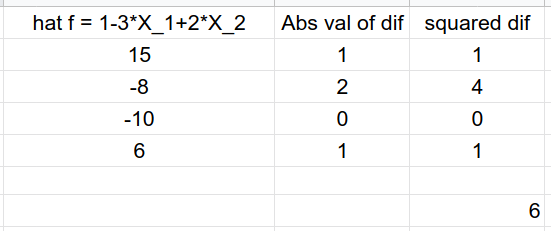
\includegraphics[alt={A table with columns hat f, absolute value of difference, and squared difference},align = c, width = \textwidth]{FakeData-Sec2-2-MSE-Soln}}
\end{columns}
\end{frame}
}
%--- Next Frame ---%


\begin{frame}[c]{Training MSE}

\begin{columns}
\column{.4\textwidth}
\centering

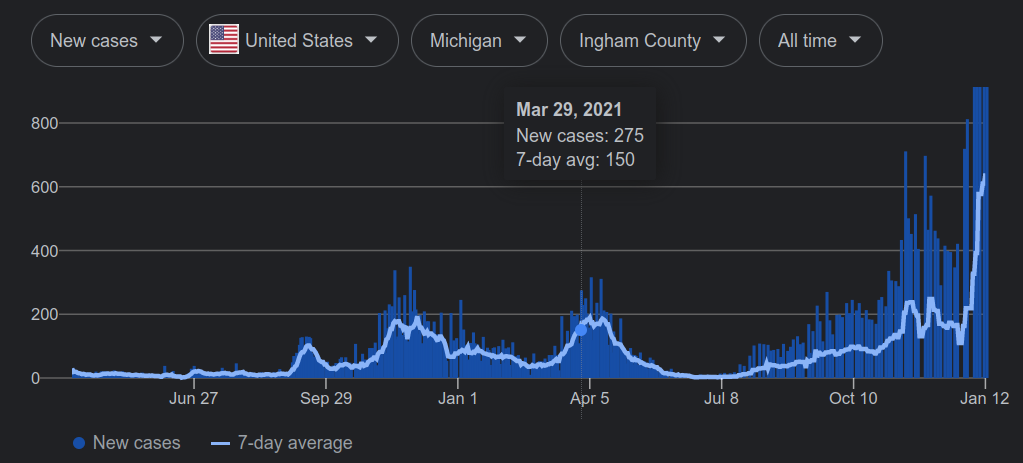
\includegraphics[alt={COVID Ingham county data in 2021},width = \textwidth]{CovidInghamCounty-Jan2022}
\column{.4\textwidth}
\centering
\InstructorNotes{We don't care about how well the model does on the data we have..... we want the quality of model on data not seen when training the model}

\end{columns}

\end{frame}
%--- Next Frame ---%


\begin{frame}[t]{Train vs test}

\begin{columns}
\column{.4\textwidth}
\centering
\textbf{Training set: }

The observations $\{(x_1,y_1),\cdots,(x_n,y_n)\}$ used to get the estimate $\hat f$
\column{.4\textwidth}
\centering

\textbf{Test set: }

The observations $\{(x_1',y_1'),\cdots,(x_{n'}',y_{n'}')\}$ used to compute the average squared prediction error
\begin{equation*}
	\frac{1}{n'}\sum_{i} (y_i' - \hat f(x_i'))^2
\end{equation*}
\end{columns}

\end{frame}
%--- Next Frame ---%


\begin{frame}[t]{Why not just get the best model for the training data?}
	\centering
	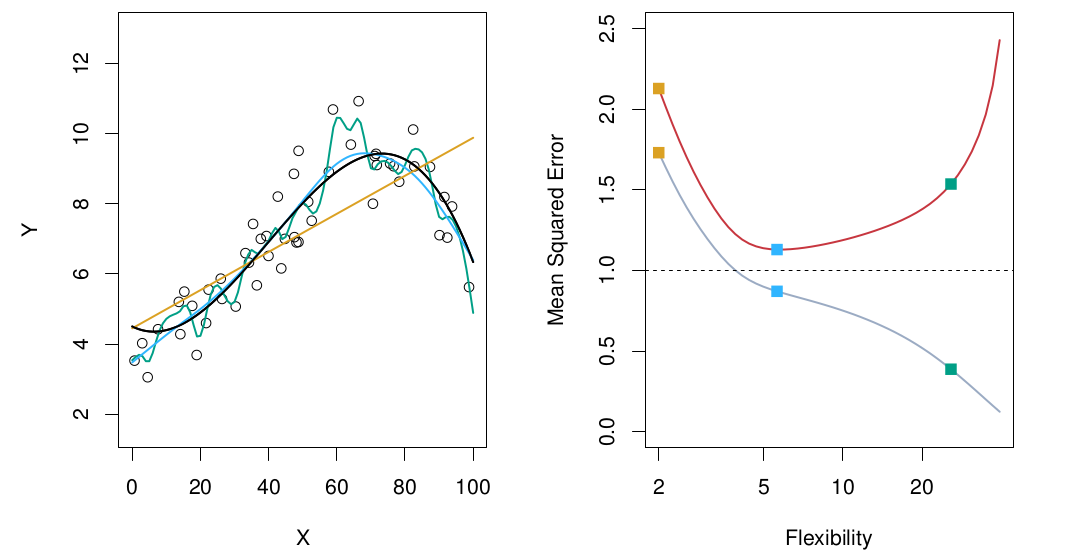
\includegraphics[alt={Plot on right is scatter plot for simulated nonlinear data with three different fits of varying flexibility. Plot on left shows the training and testing MSE as a function of flexibility},width = .7\textwidth]{Fig2-9.png}


\tiny
	\InstructorList{
	\item Left: Black line is model for simulation of data, three estimates of f are shown in orange, blue and green curves
	\item Right side: training MSE  in blue/grey, testing in red
	\item Squares represent the training and test MSEs for the three fits shown in the left-hand panel
	\item Variance of $\e$ is dashed line
	\item Point out that training error goes down but test goes up (overfitting)
	\item Flexibility = degrees of freedom
	}
\end{frame}
%--- Next Frame ---%
\begin{frame}[t]{A more linear example}
	\centering
	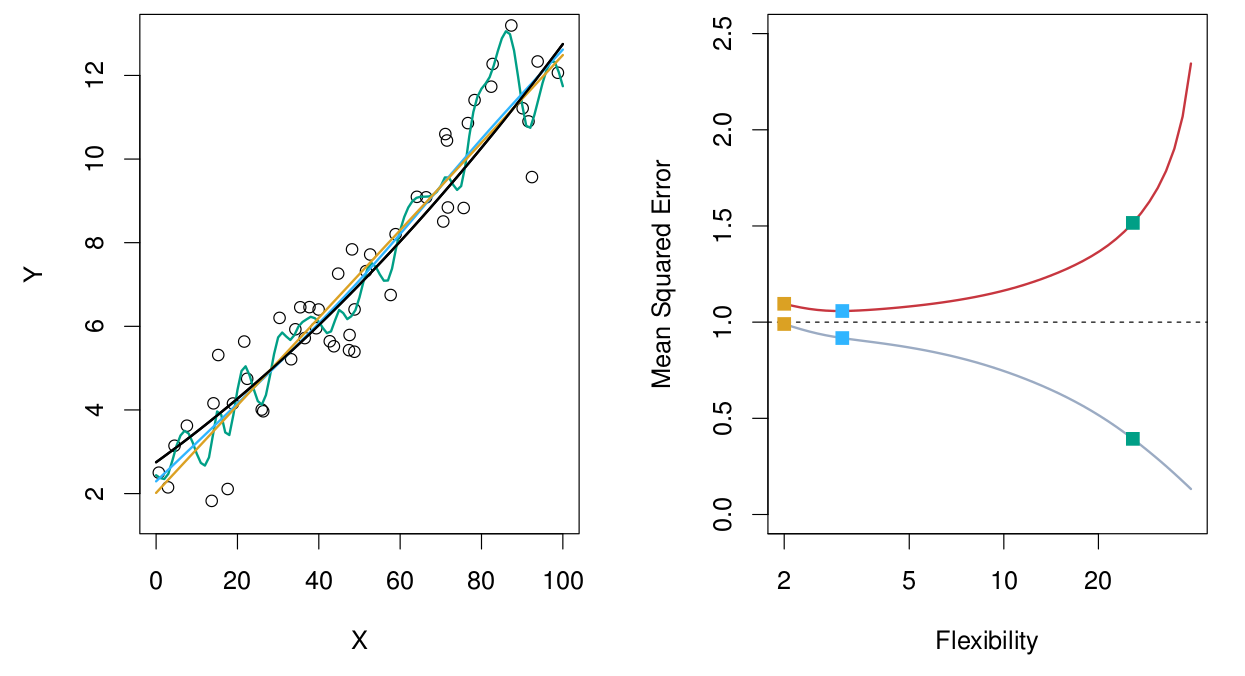
\includegraphics[alt={Plot on right is scatter plot for simulated close to linear data with three different fits of varying flexibility. Plot on left shows the training and testing MSE as a function of flexibility},width = .7\textwidth]{Fig2-10}
	\tiny
	\InstructorList{
	\item Truth is linear, so test MSE down only a bit before going up
	}
\end{frame}
%--- Next Frame ---%
\begin{frame}[t]{A more non-linear example}
	\centering
	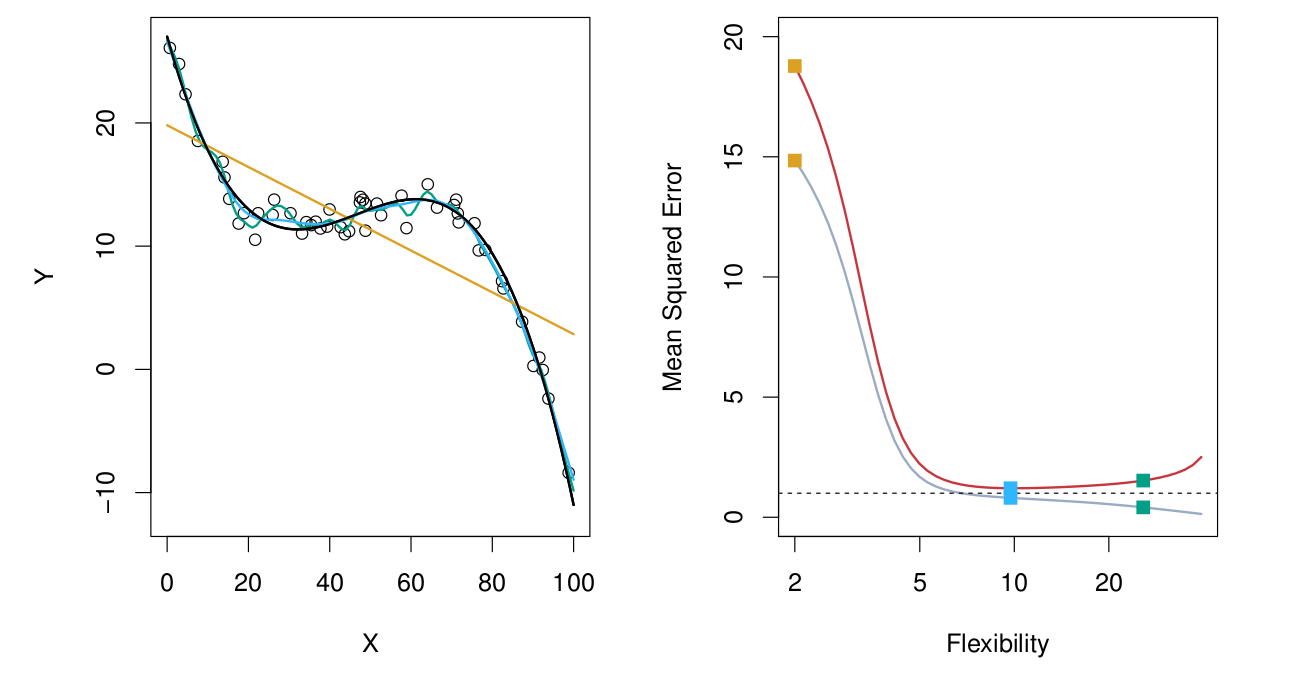
\includegraphics[alt={Plot on right is scatter plot for simulated more nonlinear data with three different fits of varying flexibility. Plot on left shows the training and testing MSE as a function of flexibility},width = .7\textwidth]{Fig2-11}
	\InstructorList{
	\item Similar structure to previous but needs more degrees of freedom before getting a good test
	}
\end{frame}
%--- Next Frame ---%
\begin{frame}[c]{A simple solution: Train/test split}
	\framesubtitle{More on this in Ch 5}

\begin{columns}
\column{.4\textwidth}
\centering

\column{.4\textwidth}
\centering

\end{columns}

\end{frame}
%--- Next Frame ---%

% \begin{frame}[c]{SOMETHING WITH GROUP WORK??}
%
% \begin{columns}
% \column{.4\textwidth}
% \centering
%
% \column{.4\textwidth}
% \centering
%
% \end{columns}
%
% \end{frame}
% %--- Next Frame ---%

%============
\section{Bias-Variance Trade-Off}
%============

\begin{frame}[t]{Bias-variance }

\begin{equation*}
	E(y_0 - \hat f (x_0))^2 = \Var(\hat f (x_0))
		+ \left[\mathrm{Bias}(\hat f(x_0)) \right] ^2
		+ \Var(\e)
\end{equation*}
\begin{columns}
\column{.4\textwidth}
\centering
\InstructorList{
\item Proof outside of the scope of class (See Bias-variance tradeoff on Wikipedia)
\item $E(y_0 - \hat f (x_0))^2$ is expected test MSE at $x_0$; avg test MSE if repeatedly estimated $f$ with lots of training sets and tested each at $x_0$
\item Computed by averaging $E(y_0 - \hat f (x_0))^2$  over all values in the test set
}
\column{.4\textwidth}
\centering
\InstructorList{
\item Eqn says we need an $\hat f$ with both low variance and low bias
\item Also says error is bounded below by irreduceable error $\Var(\e)$
}
\end{columns}


\end{frame}
%--- Next Frame ---%
\begin{frame}[c]{Variance}

\begin{columns}
\column{.45\textwidth}
% \centering
\textbf{Variance:} the amount by which $\hat f$ would change if we
estimated it using a different training data set.
\InstructorList{
\item High variance: small changes in training data result in large changes in $\hat f$.
\item Example right: green curve more flexible, but also small changes in data set could cause large changes in the computed model.
}
\column{.4\textwidth}
\centering
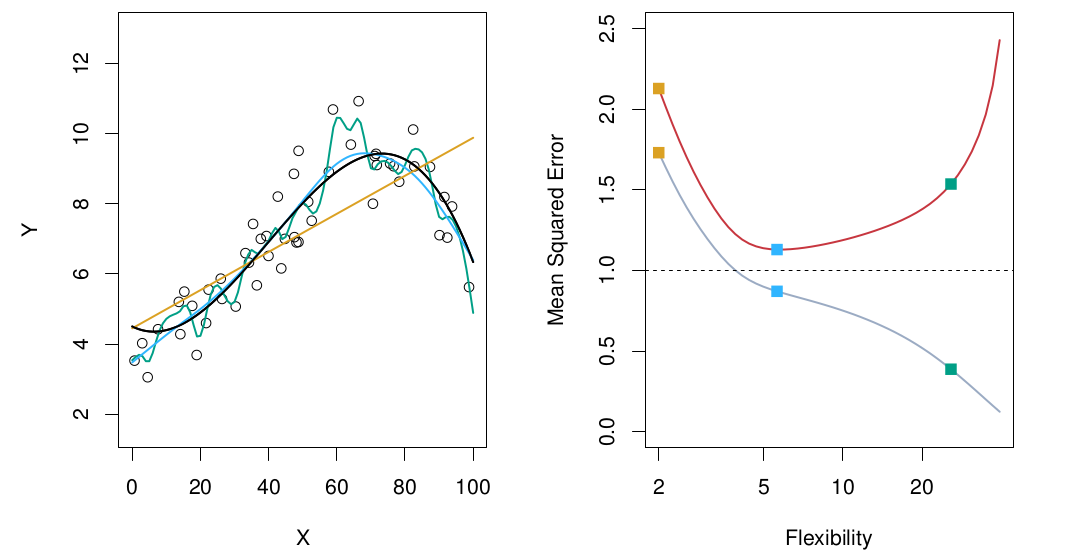
\includegraphics[alt={Scatter plot for simulated nonlinear data with three different fits of varying flexibility},width = \textwidth,clip, trim = 0 0 550 0 ]{Fig2-9}
\end{columns}

\end{frame}
%--- Next Frame ---%
\begin{frame}[t]{Bias}

\begin{columns}
\column{.45\textwidth}
% \centering

\textbf{Bias:} the error that is introduced by approximating a (complicated) real-life problem by a much simpler model.

% \tiny
\InstructorList{
\item Example: Linear regression, likely too simple for any real-life problem.
\item Figure at left: True $f$ is non-linear, so no good estimate possible with linear regression. (linear regression = high bias)
\item Figure at right: True $f$ is linear, so linear regression should do a good job (linear regression = low bias)
}
\column{.25\textwidth}
\centering
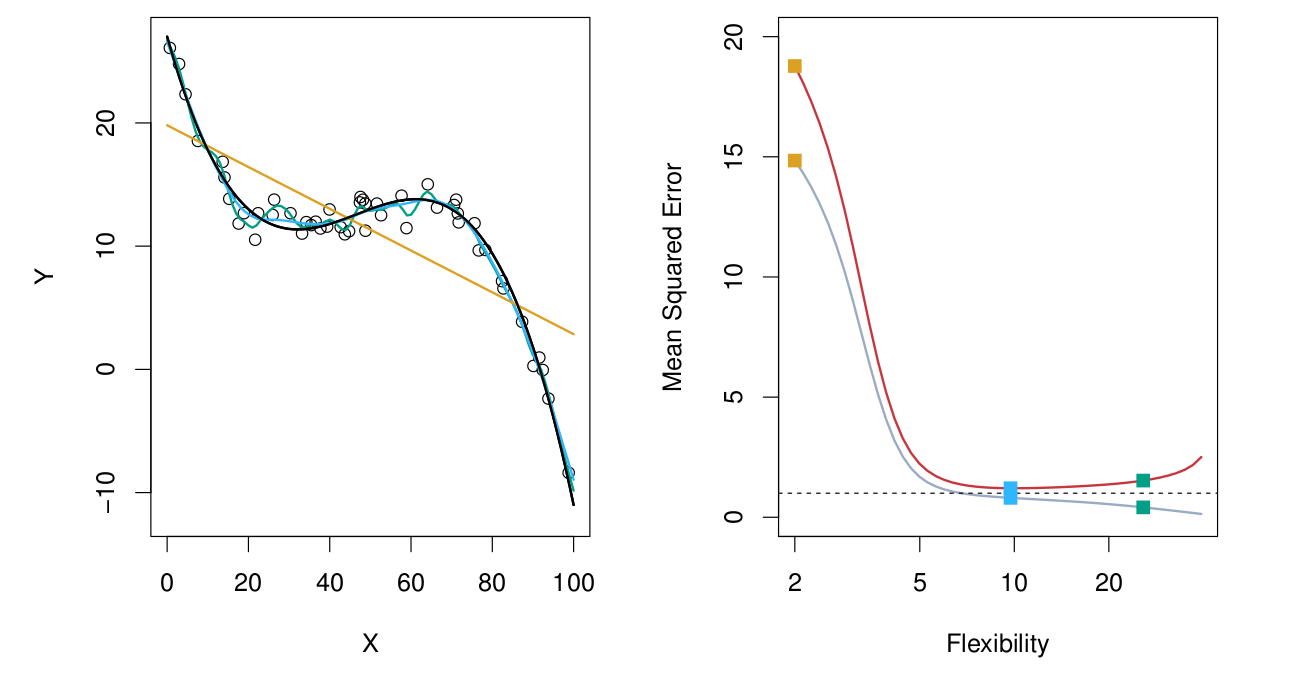
\includegraphics[alt={Scatter plot for simulated more nonlinear data with three different fits of varying flexibility},width = \textwidth,clip, trim = 0 0 700 0 ]{Fig2-11}
\column{.25\textwidth}
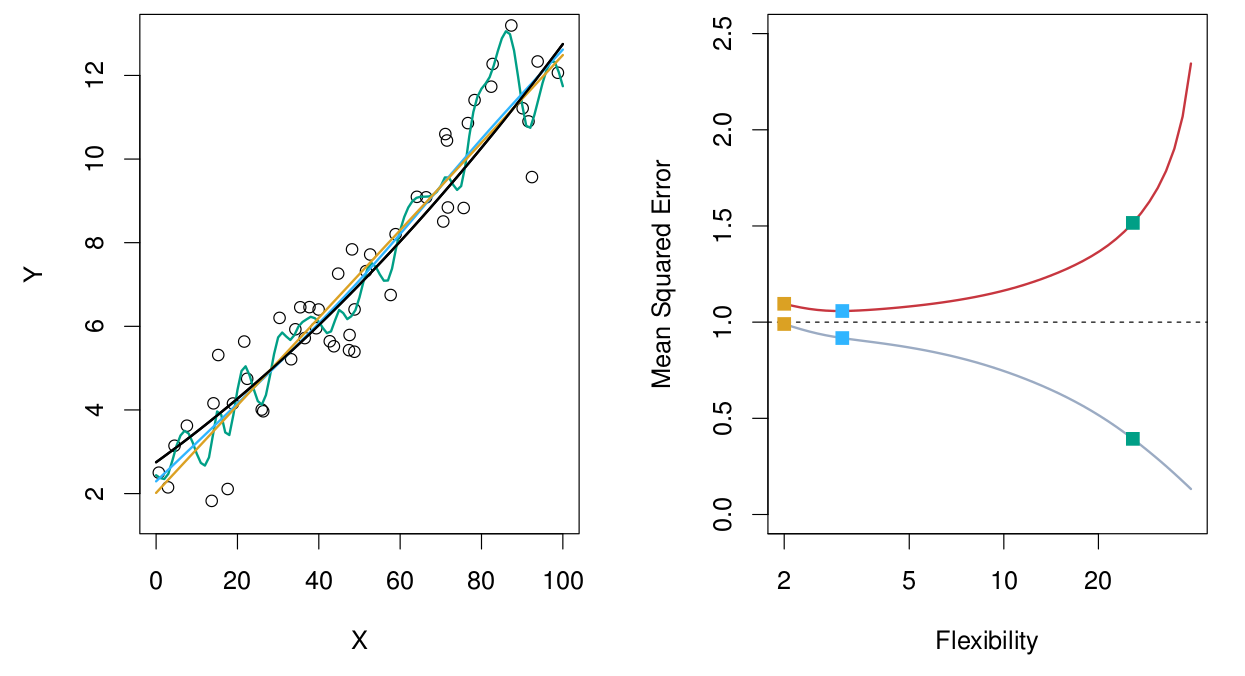
\includegraphics[alt={Scatter plot for simulated close to linear data with three different fits of varying flexibility},width = \textwidth,clip, trim = 0 0 700 0 ]{Fig2-10}

\end{columns}

\end{frame}
%--- Next Frame ---%
{
  \setbeamercolor{background canvas}{bg=Apricot!25}
\begin{frame}[c]{Group work}
	\bvfill
\begin{columns}
\column{.3\textwidth}
\centering
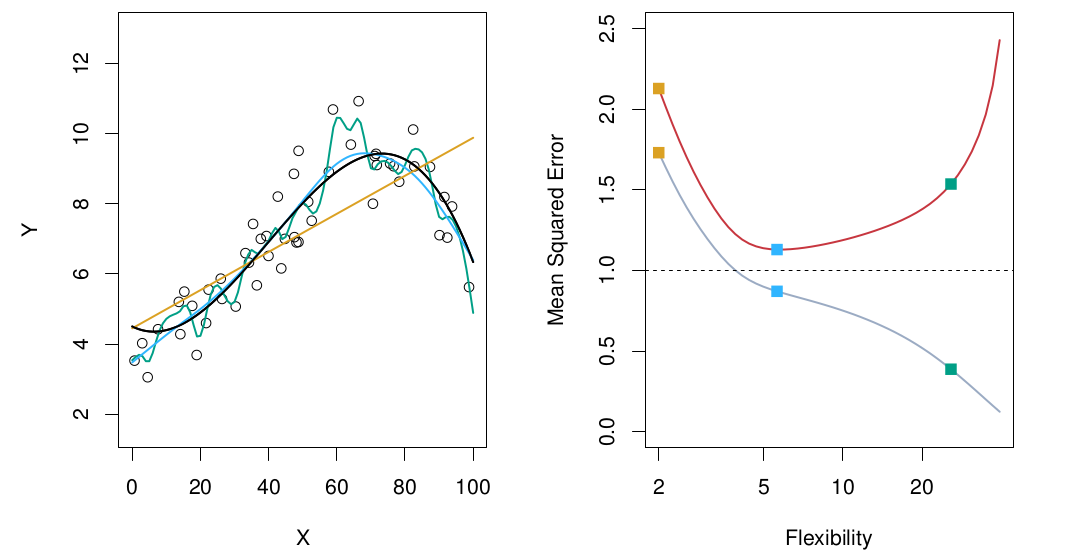
\includegraphics[alt={Scatter plot for simulated nonlinear data with three different fits of varying flexibility},width = \textwidth,clip, trim = 0 0 600 0 ]{Fig2-9}
\column{.3\textwidth}
\centering
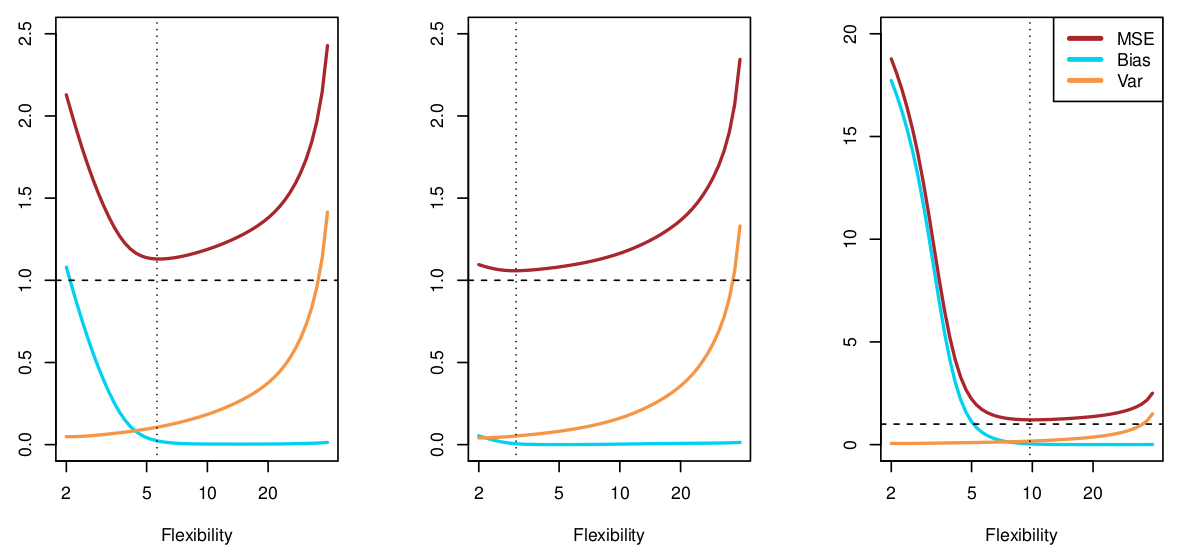
\includegraphics[alt={Three plots showing the MSE, Bias, Variance, and Variane of epsilon versus flexibility},width = .8\textwidth,clip, trim = 0 0 800 0 ]{Fig2-12}
\column{.3\textwidth}
Label the line corresponding to each of the following:
\begin{itemize}
	\item MSE 
	\item Bias 
	\item Variance of $\hat f(x_0)$
	\item Variance of $\e$
\end{itemize}
\end{columns}
	\bvfill
\begin{equation*}
	E(y_0 - \hat f (x_0))^2 = \Var(\hat f (x_0))
		+ \left[\mathrm{Bias}(\hat f(x_0)) \right] ^2
		+ \Var(\e)
\end{equation*}
\end{frame}
}
%--- Next Frame ---%


\begin{frame}[c]{Another example}
	\bvfill
\begin{columns}
\column{.3\textwidth}
\centering
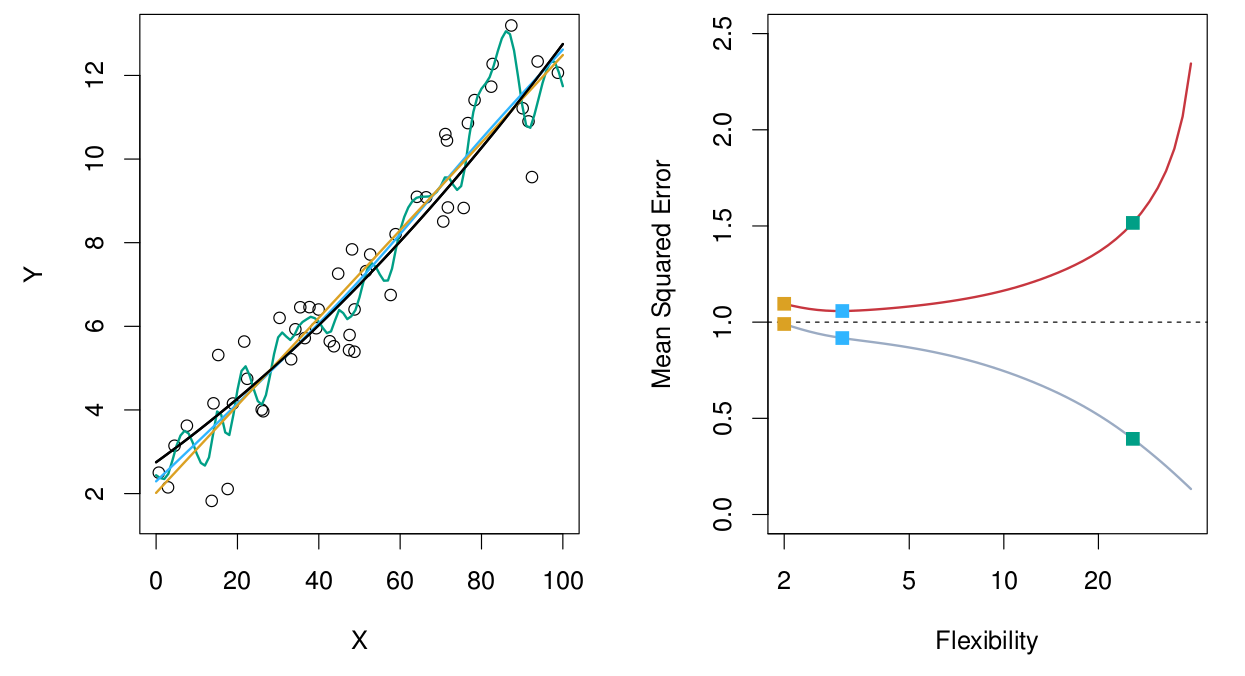
\includegraphics[alt={Scatter plot for simulated close to linear data with three different fits of varying flexibility},width = \textwidth,clip, trim = 0 0 600 0 ]{Fig2-10}
\column{.3\textwidth}
\centering
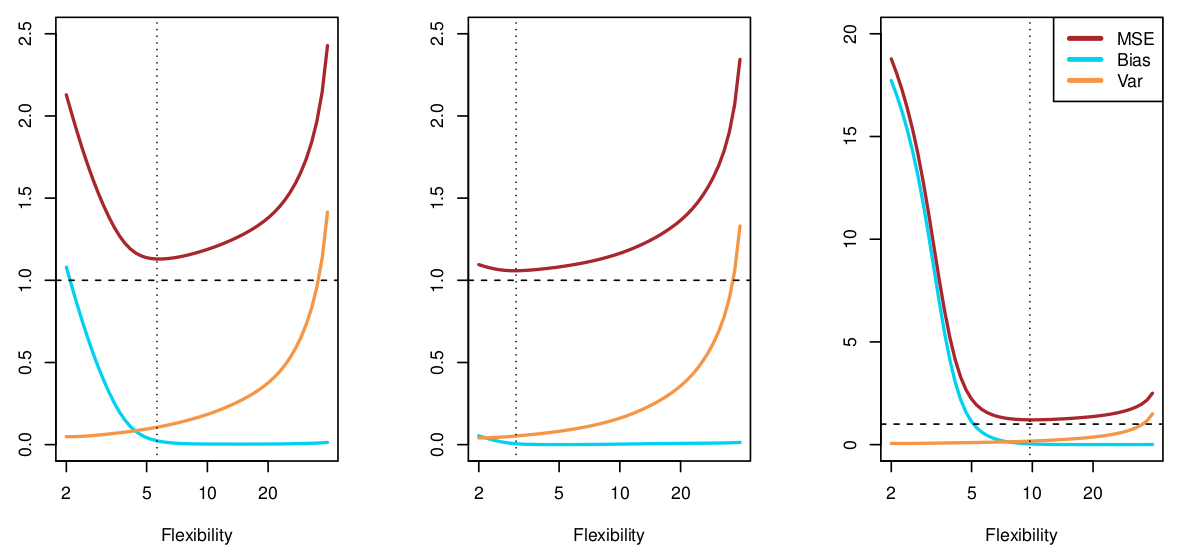
\includegraphics[alt={Three plots showing the MSE, Bias, Variance, and Variane of epsilon versus flexibility},width = .8\textwidth,clip, trim = 400 0 400 0 ]{Fig2-12}
\column{.3\textwidth}
\InstructorNotes{
Label the line corresponding to each of the following:
\begin{itemize}
	\item MSE 
	\item Bias 
	\item Variance of $\hat f(x_0)$
	\item Variance of $\e$
\end{itemize}
}
\end{columns}
	\bvfill
\begin{equation*}
	E(y_0 - \hat f (x_0))^2 = \Var(\hat f (x_0))
		+ \left[\mathrm{Bias}(\hat f(x_0)) \right] ^2
		+ \Var(\e)
\end{equation*}
\end{frame}
%----

\begin{frame}[c]{Yet another example}
	\bvfill
\begin{columns}
\column{.3\textwidth}
\centering
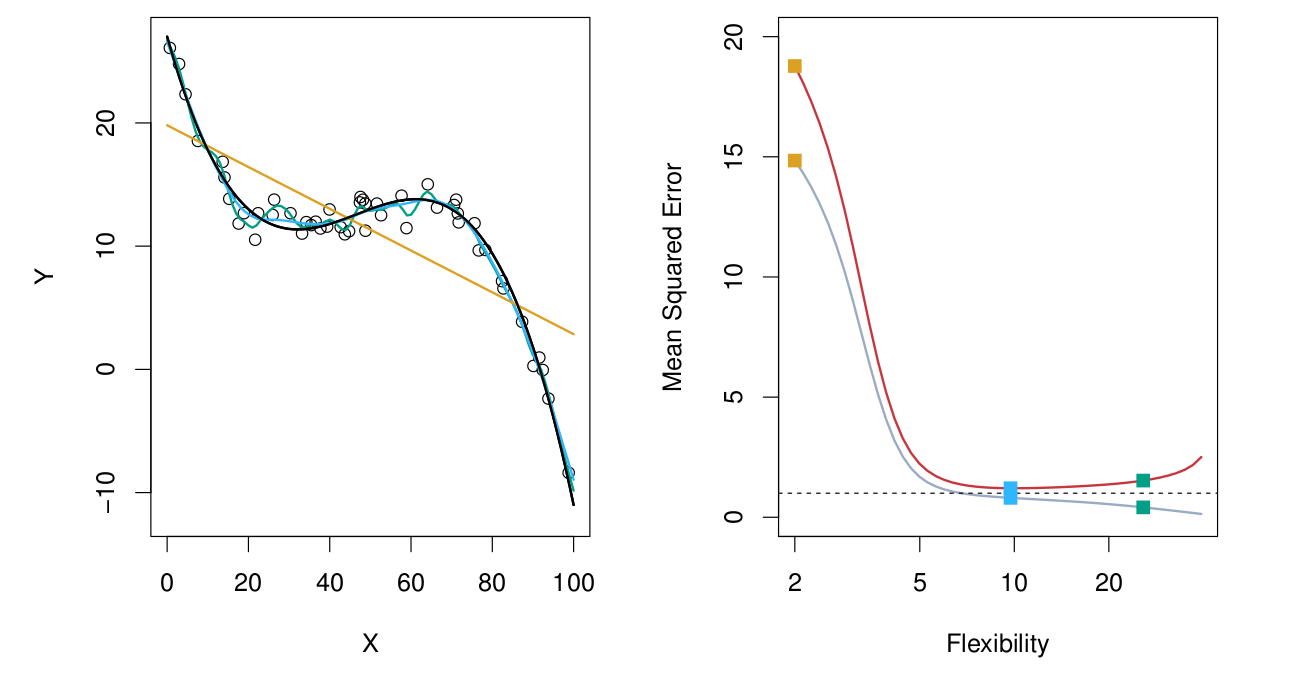
\includegraphics[alt={Scatter plot for simulated more nonlinear data with three different fits of varying flexibility},width = \textwidth,clip, trim = 0 0 600 0 ]{Fig2-11}
\column{.3\textwidth}
\centering
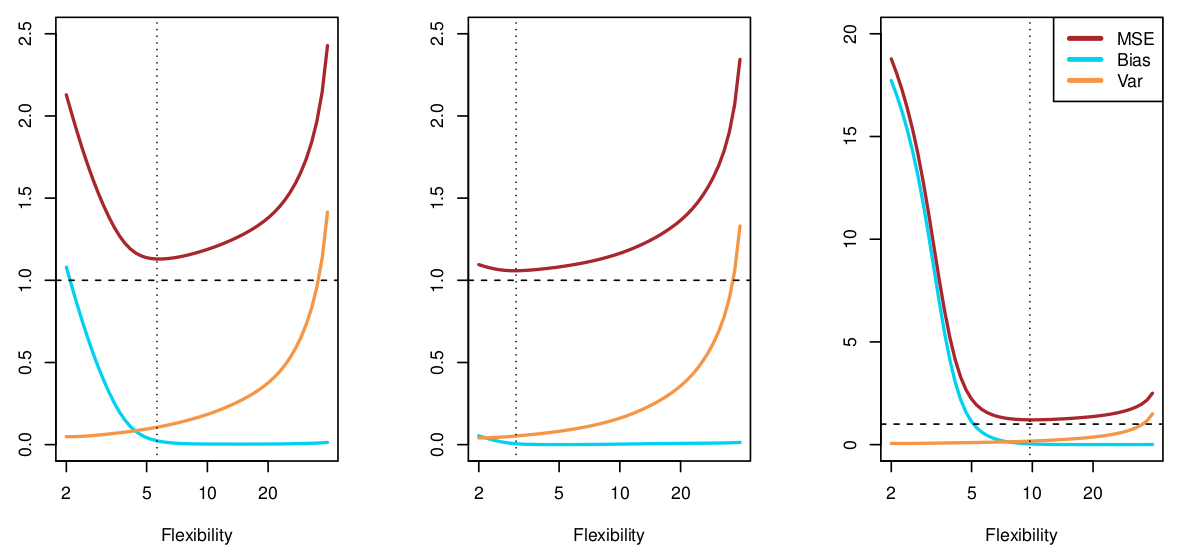
\includegraphics[alt={Three plots showing the MSE, Bias, Variance, and Variane of epsilon versus flexibility},width = .8\textwidth,clip, trim = 800 0 0 0 ]{Fig2-12}
\column{.3\textwidth}
\InstructorNotes{
Label the line corresponding to each of the following:
\begin{itemize}
	\item MSE 
	\item Bias 
	\item Variance of $\hat f(x_0)$
	\item Variance of $\e$
\end{itemize}
}
\end{columns}
	\bvfill
\begin{equation*}
	E(y_0 - \hat f (x_0))^2 = \Var(\hat f (x_0))
		+ \left[\mathrm{Bias}(\hat f(x_0)) \right] ^2
		+ \Var(\e)
\end{equation*}
\end{frame}
%----
%--- Next Frame ---%
\begin{frame}[t]{Bias-variance trade off}

	\begin{columns}
	\column{.3\textwidth}
	\centering
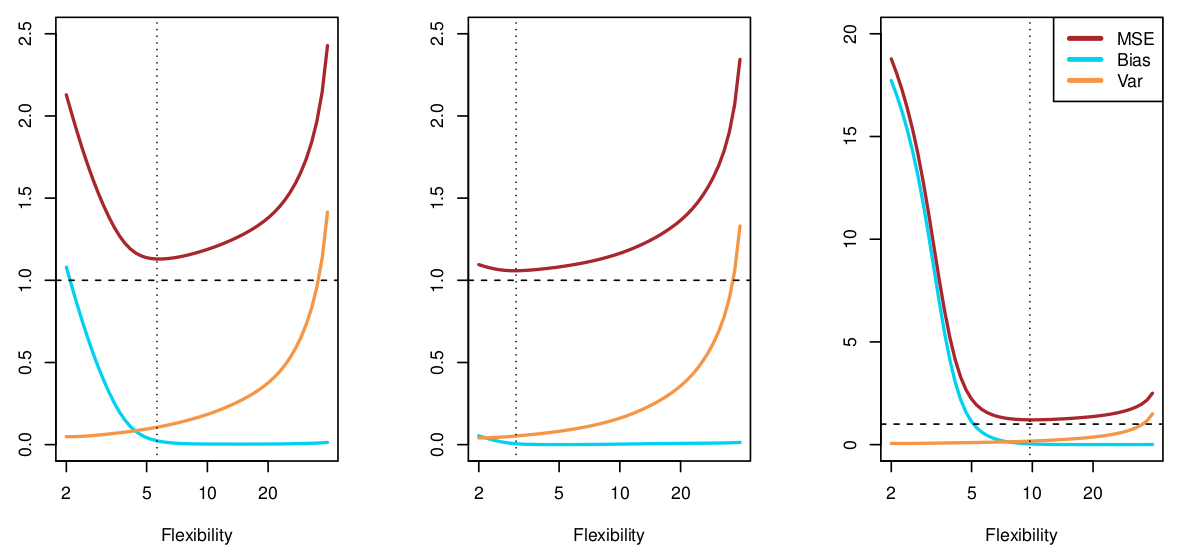
\includegraphics[alt={Three plots showing the MSE, Bias, Variance, and Variane of epsilon versus flexibility},width = .8\textwidth,clip, trim = 0 0 800 0 ]{Fig2-12}
	
	\column{.6\textwidth}
	\centering
	\InstructorList{
		\item More flexible: variance up, bias down.
		\item Relative rate of change between bias and variance determines whether MSE goes up or down
		\item Initially, bias goes down faster, so MSE declines
		\item Eventually little effect on bias but lots of increased variance, so MSE increases
	}
	\end{columns}

	\bvfill
\begin{equation*}
	E(y_0 - \hat f (x_0))^2 = \Var(\hat f (x_0))
		+ \left[\mathrm{Bias}(\hat f(x_0)) \right] ^2
		+ \Var(\e)
\end{equation*}
\end{frame}
%--- Next Frame ---%
{
  \setbeamercolor{background canvas}{bg=Apricot!25}
\begin{frame}[t]{Group work: coding}
\begin{columns}
\column{.45\textwidth}
\centering
See jupyter notebook
\column{.45\textwidth}
\centering
\end{columns}
\end{frame}
}
%--- Next Frame ---%
% %----------------
\begin{frame}[t]{Next time}

	\begin{columns}
	\column{.4\textwidth}
	\centering
	\begin{itemize}
		\item Wednesday:
		\begin{itemize}
			\item 3.1 Linear Regression
		\end{itemize}
		\item Sunday
		\begin{itemize}
			\item Homework due midnight on www.msu-stt-learning.com
		\end{itemize}
		% \item Monday:
		% \begin{itemize}
		% 	\item Ch 2.2: Assessing Model Accuracy
		% \end{itemize}

	\end{itemize}
	
	\column{.4\textwidth}
	\centering
	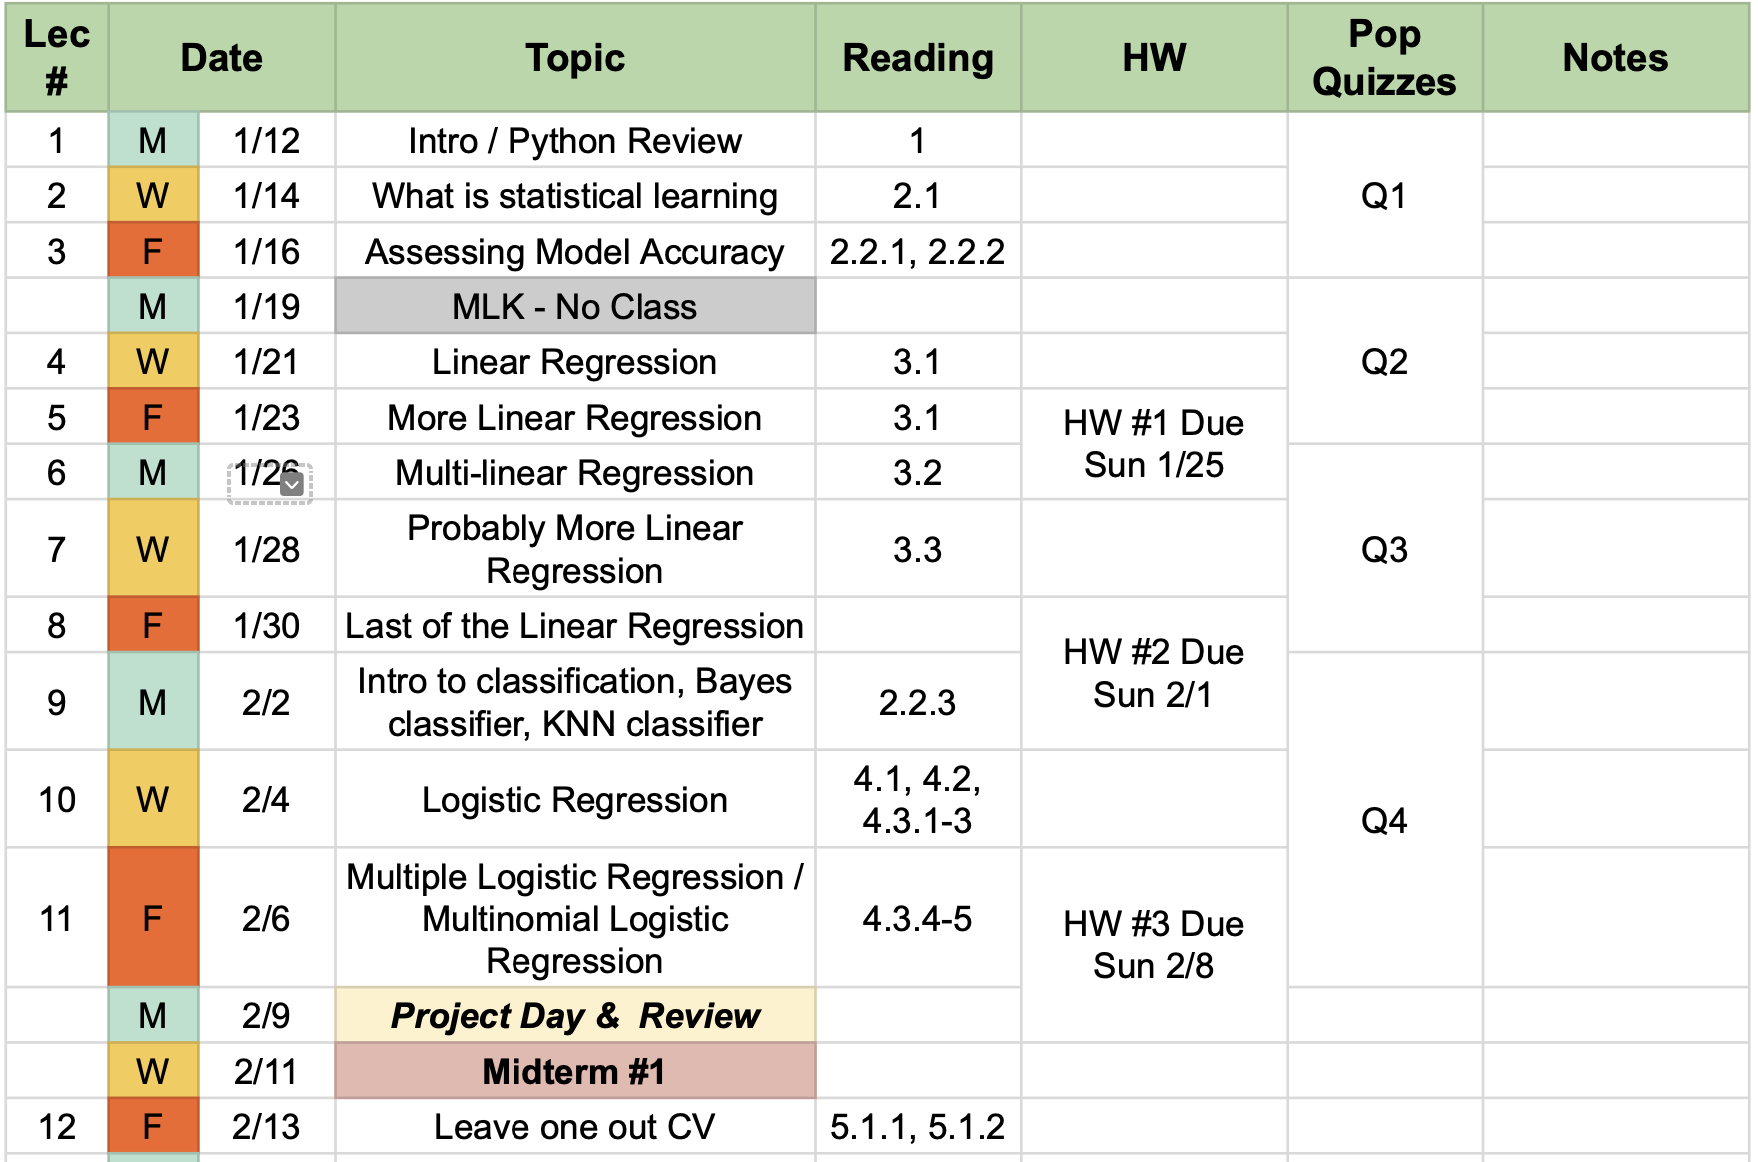
\includegraphics[alt={screenshot of course class schedule for lectures 1 to 12},align = c, width = \textwidth, trim = 0 200 0 0, clip]{Schedule-S26-1.png}
	\end{columns}

\end{frame}
%--- Next Frame ---%


\end{document}
